\documentclass{article}
\usepackage{graphicx} % Required for inserting images
\usepackage{CJKutf8}
\usepackage{amsthm}
\usepackage{mdframed}
\usepackage{float}

% 自定義 "Definition" 環境
\newmdtheoremenv{definition}{Definition}

\title{hw8}
\author{110201534 楊成偉}
\date{}

\begin{document}
\begin{CJK*}{UTF8}{bkai}
\maketitle


we will show the following graph satisfing the statement.
\begin{figure}[H]
    \centering
    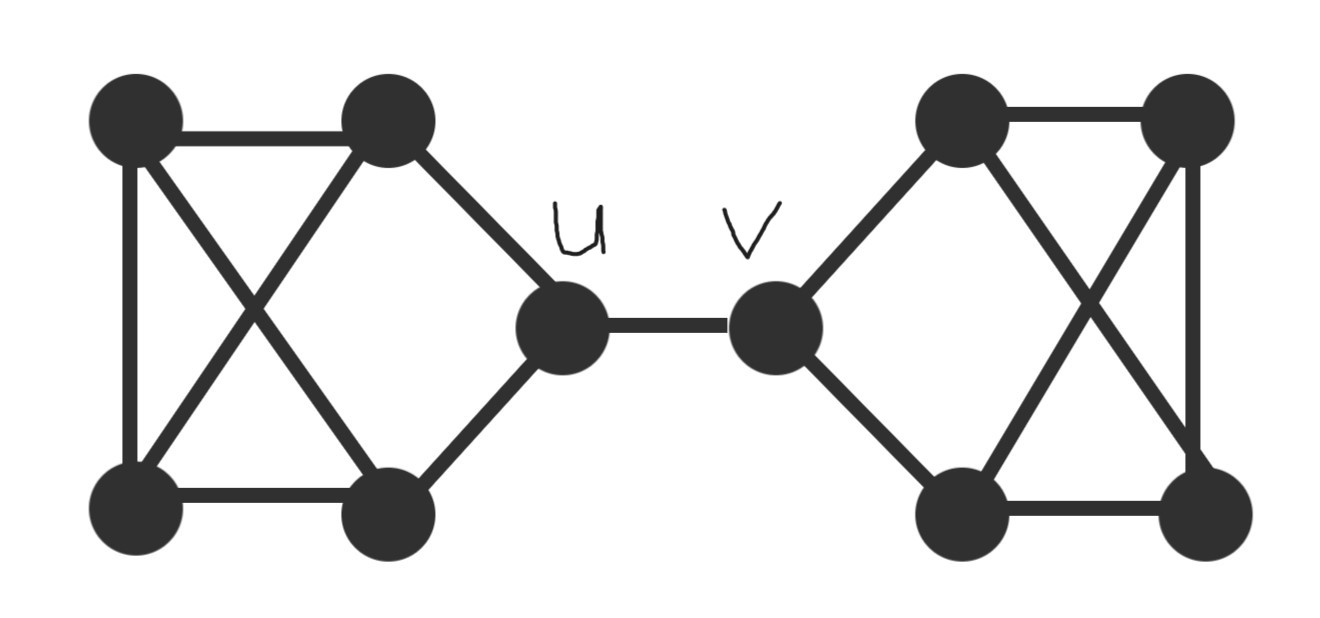
\includegraphics[scale = 0.1]{hw8g.jpg}
    \caption{A simple 3-regular graph with connectivity 1}
\end{figure}
\section*{step1}
Since the connectivity \( \kappa(G) = 1 \), it follows that there exists a vertex \( u \) that is a cut-vertex in \( G \). Because the degree of \( u \) is 3, removing \( u \) disconnects \( G \) into multiple components.

By the definition of a cut-vertex, \( u \) must connect to at least two distinct components of the resulting subgraph \( H \). Among these components, there must exist at least one component that is connected to \( u \) by exactly one edge. If we remove this edge, will make the graph be disconnected, so we have $\kappa'(G) = 1$

\section*{step2}
By connectivity is 1, so we can say that G is connected, and if we remove a cut-edge, then we get G-e have two components.
\section*{step3}
Since we only remove an edge, for each component, only the degree of the vertex that is the endpoint of the edge will decrease, while the degree of the other vertex, which has degree 3, remains unchanged.
\section*{step4}
Suppose a component with odd order, we have sum of degree of the component is odd (3*odd + even), but we know that sum of degree must be even, we get a contradiction.
\section*{step5}
Suppose there are exactly 2 vertice with degree 3 in H, but in the component, we only 3 vertice(2vertice with degree 3 and 1 vertex with degree 2), and the component is simple, so we get the contradiction.
\section*{step6}
sum of degree of H = 14 = 2*7, so we know the number of edges in H = 7, construct the following grpah, the graph shows that there can be exactly 4 vertice of degree 3 in H.
\begin{figure}[H]
    \centering
    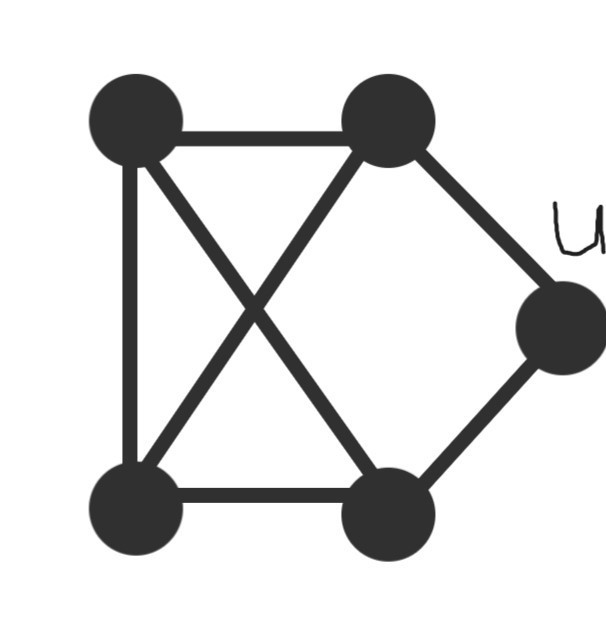
\includegraphics[scale = 0.1]{hw8gleft.jpg}
    \caption{A example for H}
\end{figure}
\section*{conclusion}
by the discussion above, we conclude that G must have 2 components, and each components have 4 vertice with degree 3, and 1 vertex with degree 2, we prove Figure 1 satisfy the statement.

\end{CJK*}
\end{document}
